%----------------------------------------------------------------------------------------
%	ABSTRACT
%----------------------------------------------------------------------------------------

\initial{Τ}{\color{teal}α προγράμματα  δέχονται δεδομένα από διάφορες εισόδους και μετά από κάποια επεξεργασία, παράγουν αποτελέσματα που εναποθέτουν στις εξόδους.
Η πιό κοινή είσοδος ονομάζεται   \textbf{standard input}  και απουσία άλλου καθορισμού αντιστοιχεί στο \textbf{πληκτρολόγιο}. Αντίστοιχα η πιο κοινή έξοδος είναι η \textbf{standard output} και απουσία άλλου καθορισμού αντιστοιχεί στην \textbf{οθόνη}. Η διοχέτευση είναι ένας τρόπος για τη σύνδεση της εξόδου ενός προγράμματος στην είσοδο ενός άλλου προγράμματος. Δυο από τα πιο δημοφιλή προγράμματα για την επεξεργασία ρεύματος είναι τα awk και sed. Τα δικαιώματα που μπορεί να έχει ένας χρήστης ή μια ομάδα χρηστών καθορίζονται με εντολές όπως η chown και η chmod.}

%----------------------------------------------------------------------------------------
%	ARTICLE CONTENTS
%----------------------------------------------------------------------------------------



%------------------------------------------------

\epigraphhead[10]{\epigraph{"UNIX is not so much an operating system as a way of thinking. "}{\textit{\href{}{}}}}

\section{Ανακατεύθυνση εισόδου - εξόδου}


Εως τώρα, οι εντολές που εκτελούσαμε έστελναν τα αποτελέσματά τους στην οθόνη. Το τερματικό  (η οθόνη) μπορεί να αντικατασταθεί από ένα αρχείο. Αν εκτελέσετε την ls σαν αποτέλεσμα θα έχει να δείτε στην οθόνη τη λίστα των αρχείων του καταλόγου που είστε. Θα μπορούσατε να ανακατευθύνετε την έξοδο της εντολής σε ένα αρχείο. Για παράδειγμα αν γράψουμε \textbf{ls $>$filelist} αυτό θα έχει σαν αποτέλεσμα να
δημιουργηθεί ένα αρχείο με όνομα \textbf{filelist} με περιεχόμενο τη λίστα των αρχείων. Το σύμβολο \textbf{$>$} σημαίνει αυτή την ανακατεύθυνση. Η συγκεκριμένη λέγεται \textbf{ανακατεύθυνση εξόδου}. Αν το αρχείο δεν υπάρχει θα δημιουργηθεί, αλλιώς τα παλιά του περιεχόμενά του θα επικαλυφθούν (override) από τα τελευταία.

Μπορούμε να συνδυάσουμε εντολές, ώστε να στείλουμε σε ένα αρχείο το περιεχόμενο άλλων αρχείων, π.χ. \textbf{cat file1 file2 file3 $>$ allfiles}. 
Αν τώρα το αρχείο της κατεύθυνσης υπάρχει και δεν θέλουμε να επικαλυφθεί, αλλά να προστεθούν τα νέα περιεχόμενα στο τέλος των παλιών, αντί για το σύμβολο \textbf{$>$} χρησιμοποιούμε το \textbf{$>>$}. 

Δημιουργήστε ένα αρχείο στον προσωπικό σας φάκελο που να περιέχει τη λίστα των αρχείων σας. Παρατηρείστε ότι το νέο αρχείο υπάρχει στη λίστα. 

Επίσης μπορούμε να ανακατευθύνουμε την είσοδο σε ένα αρχείο. Μέχρι τώρα δίναμε είσοδο από το πληκτρολόγιο. Μπορούμε να δώσουμε είσοδο σε μια εντολή από ένα αρχείο, για παράδειγμα \textbf{sort $<$ filename}. Η περίπτωση αυτή λέγεται \textbf{ανακατεύθυνση εισόδου}.  Δηλαδή το σύμβολο
\textbf{$<$} δίνει σαν είσοδο σε μια εντολή ένα αρχείο και όχι από το τερματικό. 

Πριν και μετά τους χαρακτήρες \textbf{$<$,$>$} μπορούν να τοποθετηθούν προαιρετικά κενά. 

Δοκιμάστε να μετρήσετε πόσα αρχεία έχετε στον κατάλογό σας.

Την ερμηνεία των συμβόλων $<$,$>$ όπως και των ειδικών συμβόλων που είδαμε πριν την κάνει το κέλυφος, χωρίς να καταλαβαίνουν τίποτα τα προγράμματα. Διαπιστώστε ότι οι εντολές \textbf{sort $<$filelist} και \textbf{sort filelist} παράγουν το ίδιο αποτέλεσμα. Τι θα γίνει αν
εκτελέσουμε την εντολή \textbf{wc filelist $>$ filelist} και την \textbf{dates $>$ filelist} ;

Συνήθως σε μια εντολή όπως η sort δίνουμε σαν ορίσματα ονόματα αρχείων. Τι θα γίνει αν δώσουμε σαν ορίσματα από το πληκτρολόγιο που δεν
αντιστοιχούν σε ονόματα αρχείων; Δοκιμάστε.

Τέλος να αναφέρουμε την ανακατεύθυνση εξόδου λαθών. Η σύνταξη είναι της μορφής \textbf{εντολή 2> όνομα-αρχείου}.    Ισχύει ότι και στην
περίπτωση της ανακατεύθυνσης εξόδου, μόνο που τώρα στο αρχείο εξόδου σώζονται τα
διαγνωστικά μηνύματα λάθους. Δοκιμάστε το!. Επίσης ισχύει και το $2>>$.

\emph{Σημείωση:} Στους φλοιούς sh, ksh και bash η ανακατεύθυνση λαθών γίνεται με το 2$>$ ή το 2$>>$. Στους φλοιούς csh και tcsh χρησιμοποιούμε
τα $>$\& και $>>$\&. Αυτό επίσης δουλεύει στον bash αλλά όχι στους sh και ksh. \footnote{Δείτε περισσότερα στο \href{https://goo.gl/JqJEgw}{https://goo.gl/JqJEgw} και στο \href{https://goo.gl/2PN263}{https://goo.gl/2PN263}}
%Για ανακατεύθυνση και της standard output και του standard error στο ίδιο αρχείο, χρησιμοποιούμε το 2>&1 στο τέλος της εντολής. 



\section{Διοχετεύσεις (pipes)}

Η διοχέτευση (pipe) είναι ένας τρόπος για τη σύνδεση της εξόδου ενός προγράμματος στην είσοδο ενός άλλου προγράμματος, χωρίς τη μεσολάβηση
κάποιου προσωρινού αρχείου. Για παράδειγμα για να μετρήσουμε τα αρχεία στον κατάλογό μας εκτελούσαμε \textbf{ls > temp} και  στη συνέχεια
\textbf{wc -l < temp}, φτιάχνοντας το προσωρινό αρχείο temp. Αυτός ο πλεονασμός λύνεται με τις διοχετεύσεις. Μπορούμε να συνδέσουμε
περισσότερα του ενός προγράμματα. Για παράδειγμα \textbf{who | grep it216} ή \textbf{who | grep it216 | wc -l}.

\begin{figure*}
	\centering
	%\scalebox{0.2}{\includegraphics{unix-tree.eps}}
	%\resizebox{\linewidth}{!}{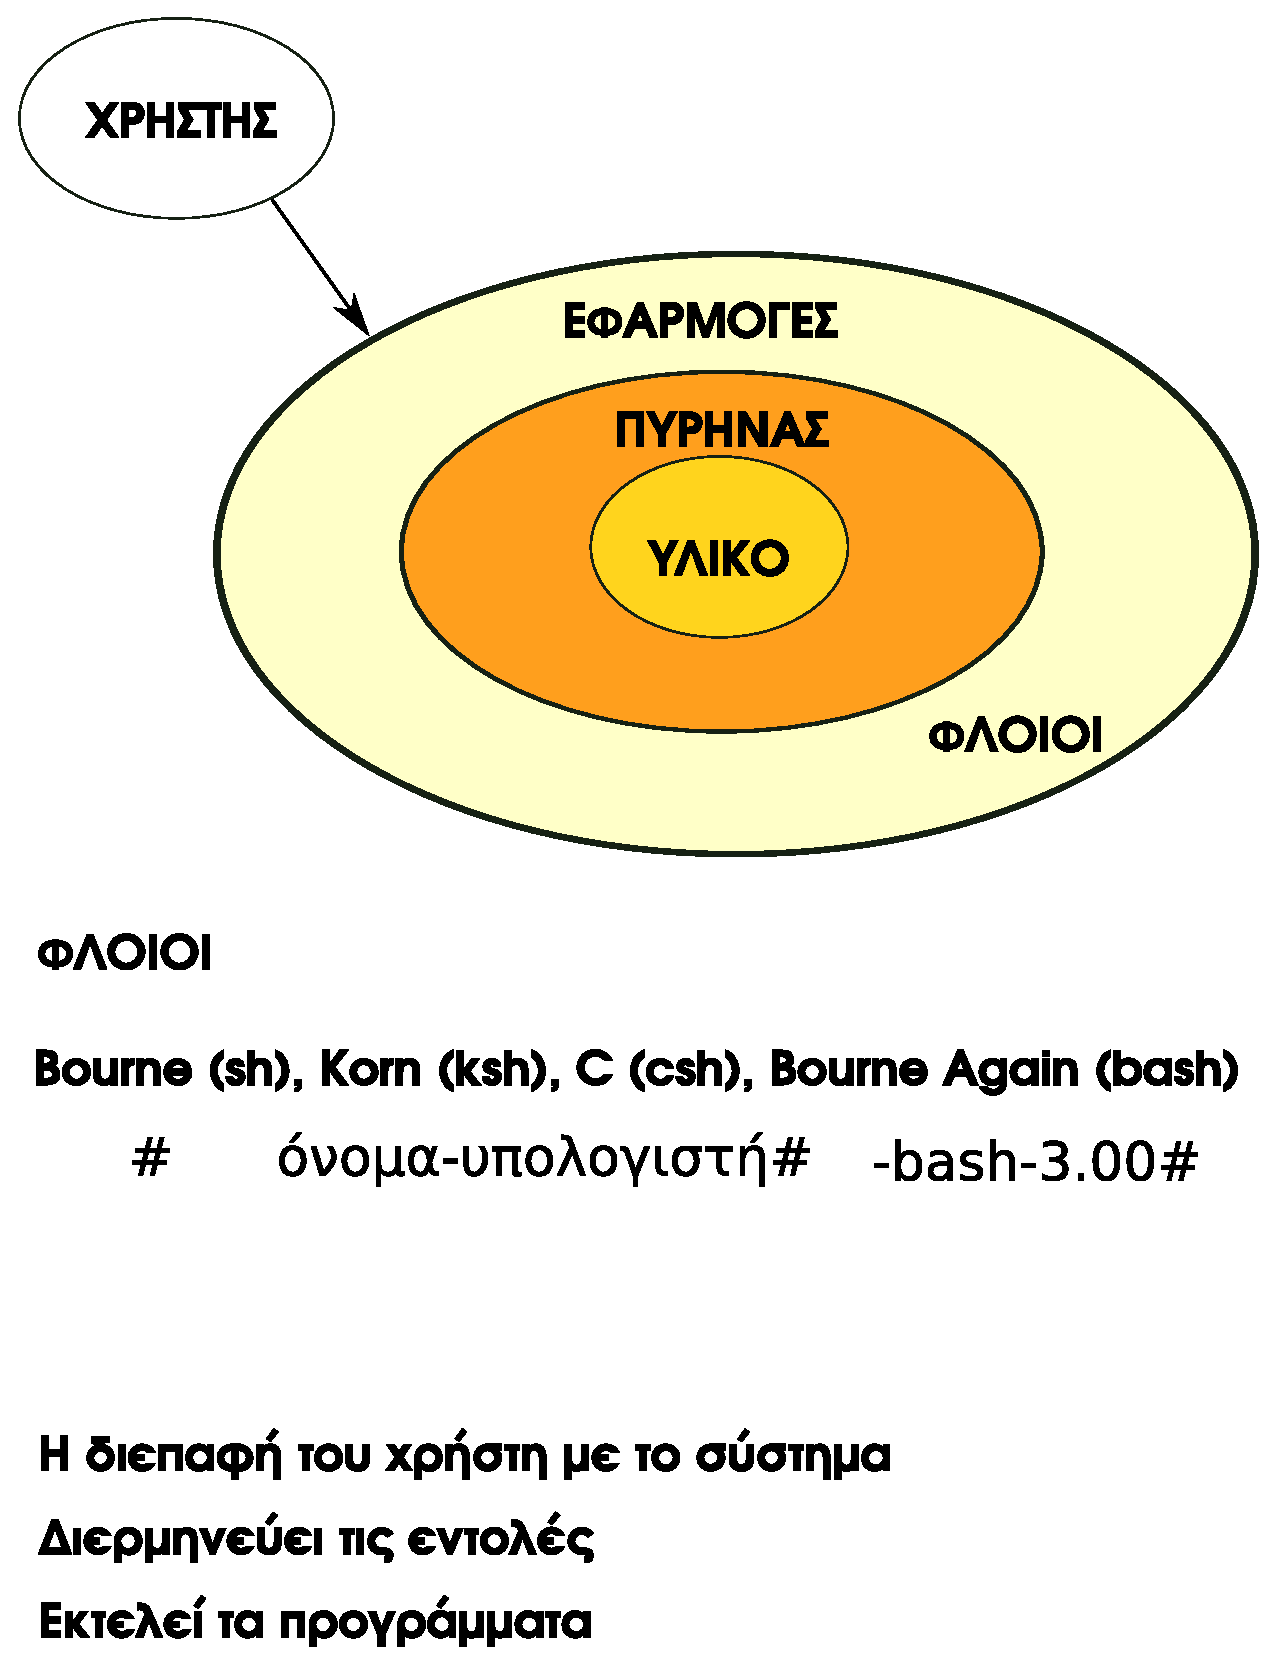
\includegraphics{shells.eps}}
	\scalebox{0.5}{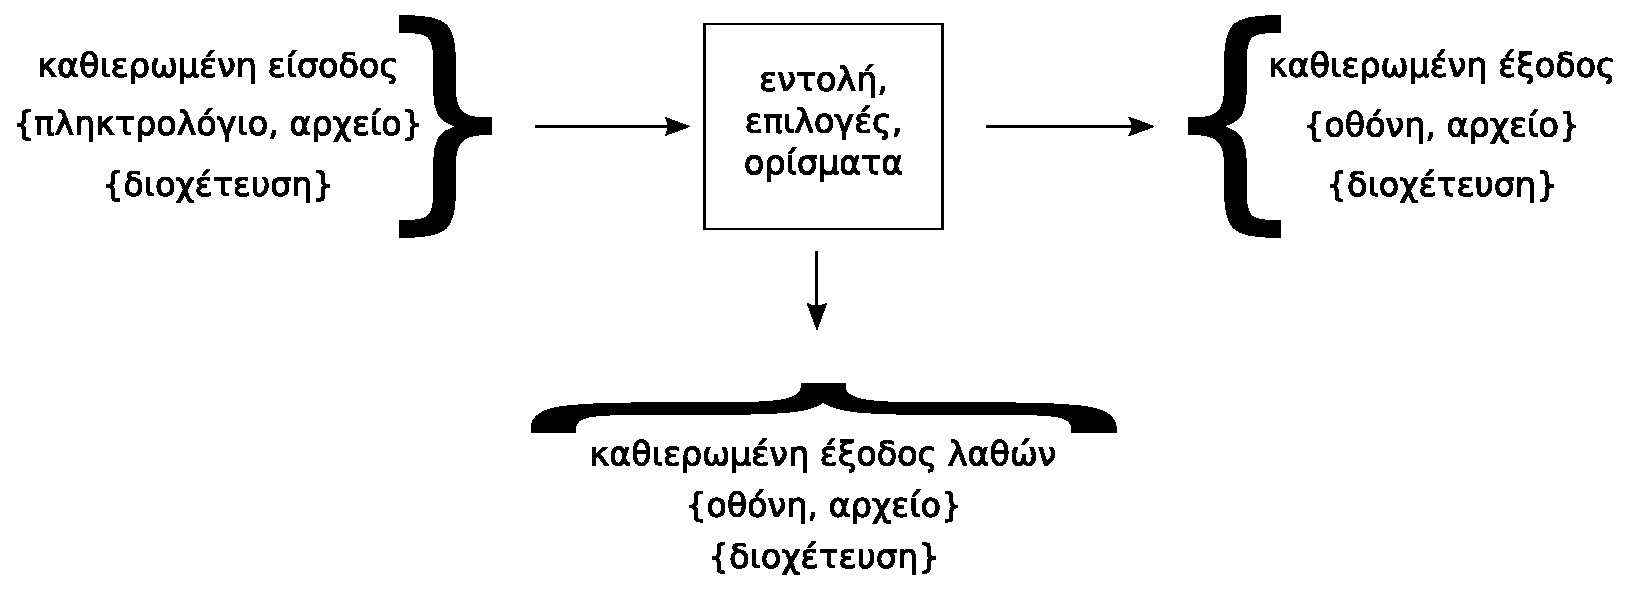
\includegraphics{images/std-in-out.eps}}
	\caption{Καθιερωμένες είσοδοι-έξοδοι}
\end{figure*} 

\subsection*{Η συνολική εικόνα} 
Οι εντολές συντάσσονται ως εξής: \\
\textbf{εντολή προαιρετικά-ορίσματα προαιρετικά-ονόματα-αρχείων}.\\
Αν δεν δοθούν ονόματα αρχείων, η εντολή διαβάζει την καθιερωμένη είσοδο (πληκτρολόγιο), αλλά μπορεί να ανακατευθυνθεί για να διαβάσει από
ένα αρχείο ή μια διοχέτευση. Στη μεριά της εξόδου οι περισσότερες εντολές γράφουν τα δεδομένα εξόδου τους στην καθιερωμένη έξοδο, εκτός αν
ανακατευθυνθούν σε κάποιο αρχείο ή διοχέτευση. Στην περίπτωση που προκύψουν μηνύματα λάθους θα πρέπει να τα ανακατευθύνουμε έτσι ούτως ώστε
να μην εμφανίζονται μέσα σε ένα αρχείο μαζί με τα αποτελέσματα της εκτέλεσης της εντολής. 

Σε μια ακολουθία διοχετεύσεων, η κάθε εντολή δέχεται είσοδο από την προηγούμενη και δίνει την έξοδό της στην επόμενη. Η πρώτη εντολή παίρνει
είσοδο από την καθιερωμένη είσοδο και η τελευταία δίνει έξοδο στην καθιερωμένη έξοδο. Σε περίπτωση που μια εντολή δεν μπορέσει να
εκτελεστεί, τότε εμφανίζονται τα μηνύματα λάθους.


\section{Άλλες χρήσιμες εντολές}

\begin{packed_item}
	\item \textbf{find}. Κάνει αναζήτηση στα περιεχόμενα ενός ή περισσοτέρων καταλόγων, μαζί με τους υποκαταλόγους τους. Πρέπει να οριστεί ο
	κατάλογος ή οι κατάλογοι αναζήτησης. Μια απλή χρήστη της find είναι: \texttt{find . -name '*.[cC]'}
	\item \textbf{cut}. Φέρνει συγκεκριμένους χαρακτήρες από κάθε γραμμή, καθορίζοντας τον πρώτο και τον τελευταίο χαρακτήρα ή καθορίζοντας
	χαρακτήρες χωρίσματος (delimiters), για παράδειγμα \texttt{who | cut -c-12} ή \texttt{cut -d ":" -f 1 /etc/passwd}.
	\item \textbf{tr}. Η εντολή tr (translate) μας παρέχει τη δυνατότητα να «μεταφράσουμε» χαρακτήρες από την standard input και να τις
	ανακατευθύνουμε στη standard output. Η γενική σύνταξη της εντολής είναι: \texttt{tr set1 set2 < stdin}. Παράδειγμα: \texttt{who | tr
		'[a-z]' '[A-Z]'}.
	\item \textbf{tar}. Δημιουργεί πακέτα αρχείων. Σε συνδυασμό με την gzip μπορεί να κάνει και συμπίεση. Παράδειγμα: 
	\begin{lstlisting}[linewidth=\columnwidth,breaklines=true]
tar -cvzf Documents.tar.gz Documents/
	\end{lstlisting}
	Προσοχή: Το πρώτο όρισμα στην tar είναι το αρχείο που θα δημιουργηθεί. Αν βάλετε κάποιο υπάρχον αρχείο, θα κάνετε \color{red}{override!!!}
\end{packed_item}

\begin{exercisebox}{ \ding{46} Ασκήσεις}
\begin{packed_enum}
	\item Εμφανίστε ταξινομημένες τις γραμμές του αρχείου /etc/passwd εμφανίζοντας μόνο το πρώτο τμήμα τους το οποίο οριοθετείται από το
	(:)
	%cut -f1 -d ':' /etc/passwd
	%cat /etc/passwd | awk '{FS=":"} { print $1}'
	\item Εμφανίστε ταξινομημένες τις γραμμές του /etc/passwd οι οποίες ξεκινούν από a ή r.
	\item Εμφανίστε αντίστροφα ταξινομημένες τις γραμμές του αρχείου /usr/share/lib/dict/words οι οποίες ξεκινούν από a ή b και έχουν μέγεθος
	μέχρι 3 γράμματα. 
	\item Μελετήστε τις εντολές uniq, comm, tee
\end{packed_enum}
\end{exercisebox}

\subsection{Ακολουθίες εντολών} 

Μπορούμε να εκτελούμε εντολές τη μια μετά την άλλη, και η σύνταξή τους είναι\\
\textbf{εντολή1; εντολή; ... εντολήΝ}. \\
Αυτές οι εντολές εκτελούνται από το δικό μας κέλυφος.

\subsection{Ομάδες εντολών}

Μπορούμε να ομαδοποιούμε τις εντολές χρησιμοποιώντας παρενθέσεις. \\
\textbf{(εντολή1; εντολή; ... εντολήΝ)}\\
Για την εκτέλεσή τους δημιουργείται ένα νεο κέλυφος. Η ομάδα εντολών μοιράζεται το ίδιο standard input και το ίδιο standard output
και μπορεί να ανακατευθυνθεί ή να διοχετευτεί σα να ήταν μια απλή εντολή. Οι παρανθέσεις έχουν παρόμοιο ρόλο με αυτόν στις
αριθμητικές παραστάσεις.


\begin{figure}
	\centering
	%\scalebox{0.2}{\includegraphics{unix-tree.eps}}
	%\resizebox{\linewidth}{!}{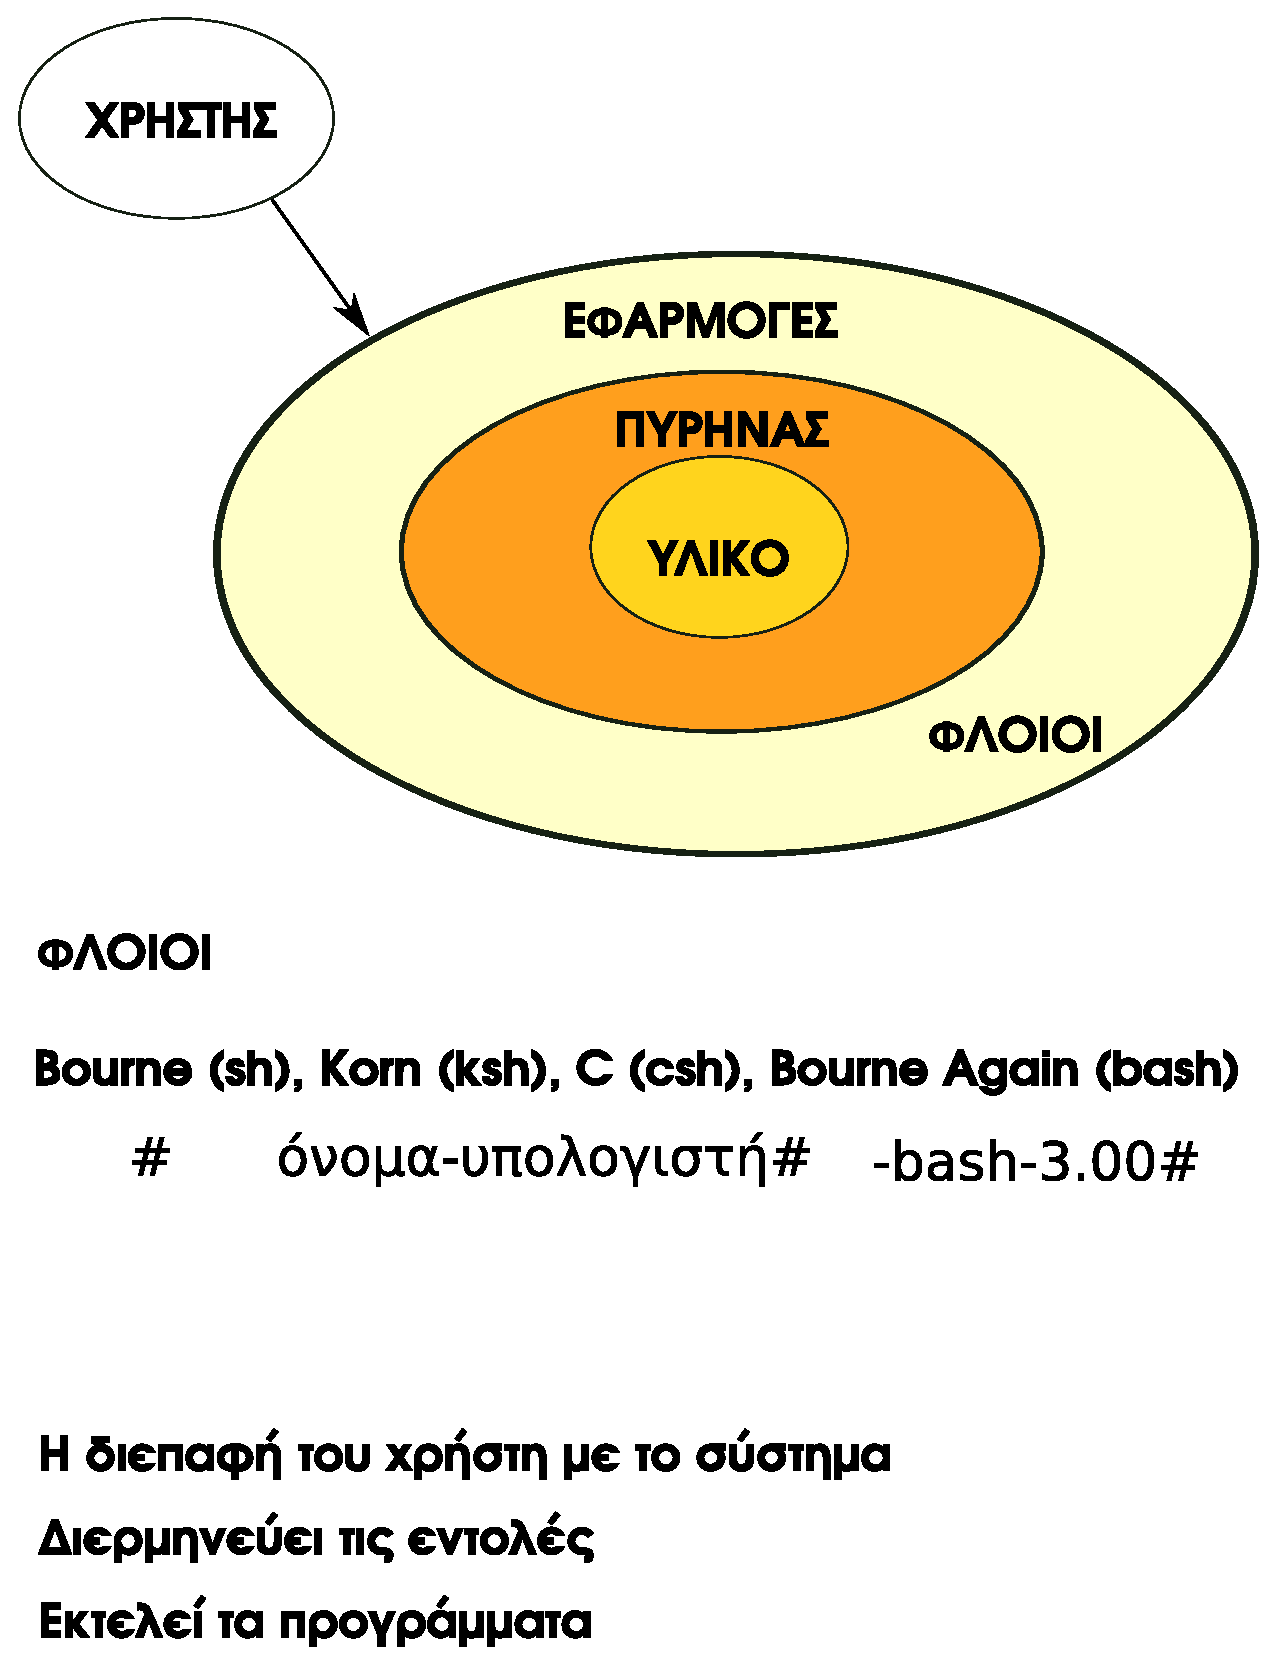
\includegraphics{shells.eps}}
	\scalebox{0.5}{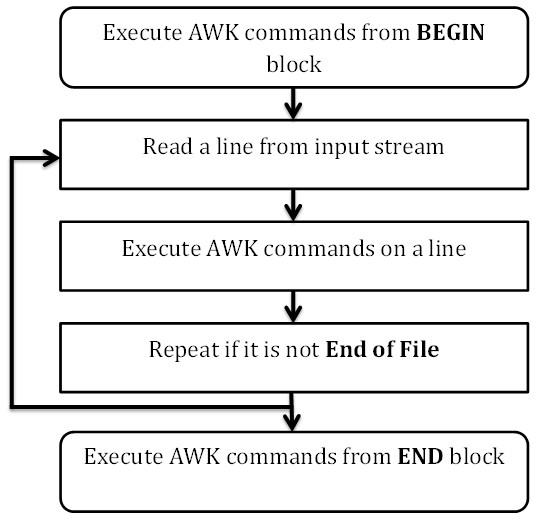
\includegraphics{images/awk_workflow.jpg}}
	\caption{awk workflow}
\end{figure} 


\section{Επεξεργασία Ρεύματος}

\subsection{awk}

Το όνομά του προέρχεται από τους Alfred \textbf{A}ho, Peter \textbf{W}einberger και Brian \textbf{K}ernighan και είναι μια γλώσσα προγραμματισμού σχεδιασμένη να εντοπίζει συγκεκριμένα πρότυπα και να εφαρμόζει σε αυτά κάποιες ενέργειες.  

Η λογική του awk είναι ότι εφαρμόζει ένα σύνολο από ενέργειες όταν βρεθεί ένα pattern.\\
\textit{pattern} '\{action\}' \\
\begin{lstlisting}
ls -lh | awk '{print $5 "\t" $9}'
\end{lstlisting}

Το awk έχει ένα σύνολο από built in variables \footnote{Δείτε στο \href{https://goo.gl/DBmkLt}{https://goo.gl/DBmkLt} και στο \href{https://goo.gl/ncKhT6}{https://goo.gl/ncKhT6}}

\subsubsection{Startup and Cleanup Actions}
Ένας BEGIN κανόνας εκτελείται μόνο μια φορά, πριν την ανάγνωση της πρώτης εγγραφής. Παρόμοια, ο κανόνας END εκτελείται μόνο μια φορά, μόλις όλο το input έχει αναγνωστεί.

\begin{lstlisting}
cat /etc/passwd |
awk 'BEGIN {FS=":";print "Start of reading"}
{++n;print  $1 }
END {print n,"rows read"}'
\end{lstlisting}

Αν θέλαμε να τυπώσουμε το χρήστη, το home directory και το default shell για κάθε χρήστη, θα γράφαμε:

\begin{lstlisting}
awk 'BEGIN{FS=":"; OFS="-"} 
{print $1,$6,$7}' /etc/passwd
\end{lstlisting}


\begin{center}
	\begin{table*}[h]
		%\footnotesize
		\begin{tabular}{ r | l }
		 ARGC & the number of arguments provided at the command line \\
		 ARGV & an array that stores the command-line arguments \\
		 CONVFMT & represents the conversion format for numbers. Its default value is \%.6g. \\
		 ENVIRON & an associative array of environment variables \\
		 FILENAME & represents the current file name \\
		 FS & represents the (input) field separator and its default value is space \\
		 NF & represents the number of fields in the current record \\
		 NR & represents the number of the current record \\
		 FNR &  similar to NR, but relative to the current file \\
		 OFMT & represents the output format number and its default value is \%.6g.\\
		 OFS & represents the output field separator and its default value is space\\
		 RLENGTH & represents the length of the string matched by match function\\
		 RS & represents (input) record separator and its default value is newline \\
		 RSTART & represents the first position in the string matched by match function \\
		 SUBSEP & represents the separator character for array subscripts and its default value is \textbackslash 034\\
		 \$0 & represents the entire input record \\	
		 \$n & represents the nth field in the current record where the fields are separated by FS\\		
		 
		\end{tabular}  
		\caption{awk built in variables} 
		\label{tab:awk_b_v}          
	\end{table*}
\end{center}
 
 
 
\subsection{sed}

Το όνομά του προέρχεται από το \textbf{S}tream \textbf{E}ditor.

\subsubsection{s for substitution}

\begin{lstlisting}
cat /etc/passwd | sed 
's/root/ADMINISTRATOR/'
\end{lstlisting}

To \textbf{s} είναι το substitute command, τα \textbf{/../../} είναι τα delimiters το πρώτο όρισμα είναι το search string ή pattern και το δεύτερο το replacement string.

Το delimiter μπορεί να αλλάξει, π.χ. σε κάτω παύλα ή άνω κάτω τελεία ή pipe character.

\subsubsection{\& για το matched string}

Το σύμβολο \& αναφέρεται στο pattern που έχει βρεθεί. Τα παρακάτω παραδείγματα αντικαθιστούν το found patter στην πρώτη περίπτωση το περικλείουν με παρενθέσεις και στη δεύτερη περίπτωση το επαναλαμβάνουν.
 
\begin{lstlisting}
echo "123 abc" | sed 's/[0-9]*/(&)/'
echo "123 abc" | sed 's/[0-9]*/& &/'
\end{lstlisting}


\subsubsection{Extended Regular Expressions}

Για να μπορέσουμε να χρησιμοποιήσουμε τα Extended RE θα πρέπει να συμβουλευτούμε το manual της sed. Συνήθως το υποστηρίζει με τη χρήση της παραμέτρου -r.

\subsubsection{Using \textbackslash 1 to keep part of the pattern}
To \textbackslash 1 αναφέρεται στο πρώτο pattern που βρέθηκε, το \textbackslash 2 στο δεύτερο κτλ. 
Για παράδειγμα αν θέλουμε να αφαιρέσουμε τους αριθμούς από μια έκφραση θα εκτελέσουμε την πρώτη εντολή ενώ αν θέλουμε να αλλάξουμε τη σειρά εμφάνισης δυο λέξεων θα εκτελέσουμε την δεύτερη εντολή\footnote{Δείτε \href{https://goo.gl/k6jzUM}{https://goo.gl/k6jzUM} την ειδική σημασία των παρενθέσεων στις κανονικές εκφράσεις όταν θέλουμε να αναφερθούμε σε pattern που έχει βρεθεί και είναι συγκεκριμένο και θέλουμε να το θυμόμαστε.}.


\begin{lstlisting}
echo abcd123 | sed 's/\([a-z]*\).*/\1/'

echo  "one two"| sed 
's/\([a-z]*\) \([a-z]*\)/\2 \1/'
\end{lstlisting}

αν θέλουμε το ίδιο να το γράψουμε χρησιμοποιώντας extended regular expressions, θα βάλουμε στην sed την παράμετρο \-r και θα αντικαταστήσουμε τα $\backslash($ με $($ και τα $\backslash)$ με $)$.

\begin{lstlisting}
echo abcd123 | sed -r 's/([a-z]*).*/\1/'

echo  "one two"| sed -r
's/([a-z]*) ([a-z]*)/\2 \1/'
\end{lstlisting}


Παράδειγμα: Πως θα βρω λέξεις οι οποίες έχουν τρια γράμματα από τα οποία το μεσσαίο είναι το o και το πρώτο είναι το ίδο με το τελετυαίο;

\begin{lstlisting}
sed -E -n '/^(.)o\1$/p' 
/usr/share/dict/words
\end{lstlisting}

Η παράμετρος -Ε είναι ίδια με το -r ενώ η παράμετρος -n σημαίνει ότι θα τυπώσει μόνο τα patterns που βρήκε κι όχι όλα τα δεδομένα που επεξεργάστηκε \href{https://goo.gl/p7qErM}{https://goo.gl/p7qErM}.
\subsubsection{Sed Pattern Flags}
\paragraph{/g: Global Replacement}
Το sed αντικαθιστά το πρώτο pattern που θα βρει (σε μια γραμμή). Αν θέλουμε να αλλάξουν όλα τα occurences θα πρέπει να χρησιμοποιήσουμε το g μετά το τελευταίο delimiter.

\begin{lstlisting}
echo  "one two three"| 
sed 's/[^ ][^ ]*/(&)/'

echo  "one two three"| 
sed 's/[^ ][^ ]*/(&)/g'
\end{lstlisting} 

\paragraph{/1, /2, etc : Specifying which occurrence}
Χωρίς flag το πρώτο pattern που ταιριάζει αλλάζει με τη sed. Aν θέλουμε να αλλάξουμε π.χ. το δεύτερο matched pattern τότε 
\begin{lstlisting}
echo "one two three four"| 
sed 's/[a-zA-Z]* / /2'
\end{lstlisting}
Θα πρέπει να δοθεί προσοχή ώστε να μην μπερδέυετε το /2 με το \textbackslash 2. To /2 μπαίνει στο τέλος ενώ το \textbackslash 2 μπαίνει στο replacement string.

\paragraph{/p: print}
Με την παράμετρο /p μετά το τελευταίο delimiter μπορούμε να χρησιμοποιήσουμε την sed ώστε να μας επιστρέψει μόνο τις γραμμές που έχουν το pattern χρησιμοποιώντας επιπλέον και την παράμετρο -n στο sed.

\begin{lstlisting}
sed -n '/root/p' /etc/passwd
\end{lstlisting} 


\paragraph{d for delete}
Το pattern είναι της μορφής \textit{[address1[,address2]]d}. Το address μπορεί να είναι είτε αριθμός γραμμής είτε κάποιο pattern. Η πρώτη εντολή σβήνει τις γραμμές 1 έως 5 από το αρχείο /etc/passwd ενώ η δεύτερη αυτές οι οποίες ξεκινάνε με n \footnote{\href{https://goo.gl/eEWdNb}{https://goo.gl/eEWdNb}}.

\begin{lstlisting}
sed '1, 5 d' /etc/passwd
sed '/^n/d' /etc/passwd 
\end{lstlisting}
 

Παραδείγματα μπορείτε να βρείτε στα ακόλουθα link:
\begin{itemize}
	\item \href{http://www.theunixschool.com/p/awk-sed.html?m=1}{theunixschool}
	\item \href{http://blog.commandlinekungfu.com/2012/12/awk-ward.html?m=1}{commandlinekungfu}
\end{itemize}


\section{Χρήστες, ομάδες και δικαιώματα}

Κάθε αρχείο ανήκει σε ένα χρήστη. Κάθε χρήστης έχει ένα μοναδικό αριθμό που τον χαρακτηρίζει (user ID - UID – User Identification). Κάθε
χρήστης μπορεί να δει μόνο τα δικά του αρχεία (ανάγνωση, εγγραφή, εκτέλεση), εκτός αν του δώσουν δικαιώματα οι άλλοι χρήστες στα δικά τους.
Κάθε αρχείο ανήκει και σε μία ομάδα. Κάθε χρήστης ανήκει σε μία τουλάχιστον ομάδα. Οι ομάδες έχουν μοναδικούς αριθμούς που τις χαρακτηρίζουν
(group ID - GID – Group Identification). Οι χρήστες μίας ομάδας μοιράζονται τα αρχεία που ανήκουν στην ομάδα. Η πρωτεύουσα ομάδα είναι
σημαντική γιατί είναι αυτή στην οποία ανήκει ένα νέο αρχείο του χρήστη που το δημιουργεί. 

Κάθε αρχείο ανήκει σε ένα χρήστη και κάθε χρήστης βλέπει τα δικά του αρχεία. Μόνο αν ο ιδιοκτήτης ενός αρχείου μας δώσει άδεια μπορούμε να
δούμε τα αρχεία του. Η ταυτότητα του χρήστη προσδιορίζεται κατά τη διαδικασία του login. Κάθε αρχείο είναι συσχετισμένο με μία ομάδα. Κάθε
διεργασία έχει ένα ιδιοκτήτη (χρήστη) και μία συσχετισμένη ομάδα, μπορεί δε να προσπελάσει μόνο τους πόρους του συστήματος που μπορεί να
προσπελάσει ο ιδιοκτήτης της και η ομάδα αυτή.

Για κάθε αρχείο και κατάλογο ορίζονται δικαιώματα πρόσβασης. Τα δικαιώματα ορίζονται για (α) τον ιδιοκτήτη (owner ή συνήθως user), (β) την
ομάδα του χρήστη (group) και (γ) για όλους τους υπόλοιπους χρήστες (others). Τα δικαιώματα είναι: ανάγνωση, εγγραφή και εκτέλεση.

Όταν μία διεργασία ζητά πρόσβαση σε ένα αρχείο, ο χρήστης και η ομάδα της διεργασίας συγκρίνονται με το χρήστη και την ομάδα του αρχείου: 
(α) Αν ο χρήστης ταυτίζεται, εφαρμόζονται τα δικαιώματα πρόσβασης του χρήστη και δεν εξετάζονται τα δικαιώματα της ομάδας και των υπολοίπων
χρηστών
(β) Αλλιώς, αν ταυτίζεται η ομάδα, εφαρμόζονται τα δικαιώματα πρόσβασης της ομάδας και δεν εξετάζονται τα δικαιώματα των υπολοίπων χρηστών
(γ) Αλλιώς, εφαρμόζονται τα δικαιώματα για τους υπόλοιπους χρήστες

Τα δικαιώματα πρόσβασης μπορούν να εμφανιστούν με χρήση της εντολής ls -l. Ο τύπος του αρχείου και τα δικαιώματα του αρχείου συμβολίζονται
με μία συμβολοσειρά 10
χαρακτήρων. Ο πρώτος χαρακτήρας αντιπροσωπεύει τον τύπο του αρχείου, οι υπόλοιποι εννέα τα δικαιώματα του αρχείου. Αν ο πρώτος χαρακτήρας
είναι d αναφερόμαστε σε
κατάλογο, αν – είναι συνηθισμένο αρχείο (υπάρχουν και άλλοι τύποι αρχείων).\\
παράδειγμα: 
\begin{lstlisting}
drwxr-xr-x   2 root     root         512 Oct 11 10:28 Desktop
\end{lstlisting}



Για να αλλάξουμε τα δικαιώματα πρόσβασης σε ένα αρχείο ή φάκελο, χρησιμοποιούμε την εντολή chmod. Συντάσσεται με δύο τρόπους:
\begin{center}
	chmod τριψήφιος-οκταδικός-αριθμός filename\\
	ή\\
	chmod [user\_specifier] mode\_change\_specifier filename
\end{center}

Στην πρώτη περίπτωση υπάρχουν οι εξής κανόνες: το πρώτο ψηφίο αναφέρεται στον ιδιοκτήτη, το δεύτερο στο group και το τρίτο στους υπόλοιπους.
Σε κάθε ψηφίο
προσθέτουμε 4 αν θέλουμε να δώσουμε δικαίωμα ανάγνωσης, 2 αν θέλουμε να δώσουμε δικαίωμα εγγραφής και 1 αν θέλουμε να δώσουμε δικαίωμα
εκτέλεσης.
Στη δεύτερη περίπτωση ο (προαιρετικός) user\_specifier καθορίζει σε ποιον εφαρμόζεται η αλλαγή των προνομίων (u = owner, g = group, o =
other) και το mode\_\-change\_specifier δείχνει ποια αλλαγή θα επέλθει (+r, -r, +w, -w, +x, -x). \\

Παραδείγματα:\\
\textbf{chmod 740 myfile}\\
δίνουμε όλα τα δικαιώματα στον ιδιοκτήτη, δικαίωμα ανάγνωσης στο group και κανένα δικαίωμα στους υπόλοιπους.\\
\textbf{chmod +x myfile} \\
δίνουμε δικαίωμα εκτέλεσης σε όλους (ή μόνο στον ιδιοκτήτη) στο αρχείο myfile. Το δικαίωμα εκτέλεσης σε έναν κατάλογο έχει το νόημα ότι
μπορούμε να κινηθούμε
μέσα σε αυτό.\\
\textbf{chmod o-w myfile}\\
αφαιρούμε το δικαίωμα εγγραφής από τους χρήστες που δεν ανήκουν στο δικό μου group από το αρχείο myfile.\\

Με τις εντολές chown και chgrp μπορούμε να μεταβιβάσουμε σε άλλους την ιδιοκτησία ενός χρήστη ή μιας ομάδας χρηστών πάνω σε μια ομάδα
αρχείων και καταλόγων. Η σύνταξη των εντολών αυτών έχει τη μορφή:\\
\textbf{chown owner file} \\
\textbf{chgrp group file} \\
όπου file είναι μια ομάδα αρχείων και καταλόγων που θέλετε να αλλάξετε την ιδιοκτησία τους.\\

Ανατρέξτε στο manual των εντολών chmod και chown για περισσότερες πληροφορίες.

\subsection*{Umask}

Όταν ένας χρήστης δημιουργεί έναν κατάλογο στο σύστημα αρχείων του UNIX, αυτό δημιουργείται με προκαθορισμένες ρυθμίσεις.

Η προκαθορισμένη ρύθμιση για τη δημιουργία αρχείων (user file-creation mode mask -umask-) χρησιμοποιείται για να καθορίσει τα δικαιώματα των δημιουργηθέντων αρχείων.


H εντολή umask δίνει τα δικαιώµατα που αφαιρούνται αυτόµατα από τα αρχεία και τους
καταλόγους που δηµιουργεί ένας χρήστης.

\begin{center}
	\begin{table}[h]
		\small
		\begin{tabularx}{\textwidth}{r|l}
			\rowcolor[gray]{0.9}
			Octal valuer	&	Permission \\
			0 & read, write and execute \\
			1 & read and write \\
			2 & read and execute \\
			3 & read only \\
			4 & write and execute \\
			5 & write only \\
			6 & execute only \\
			7 & no permissions \\
		\end{tabularx}  
		\caption{οκταδικά umasks} 
		\label{tab:operators}          
	\end{table}
\end{center}

Πως υπολογίζονται: Αν για παράδειγμα το umask είναι 0022\footnote{Το επιπλέον ψηφίο μπροστά από τα 3 ψηφία έχει ειδική σημασία, 4000 = SUID, 2000 = SGID, 1000 = sticky bit, δείτε \href{http://docs.oracle.com/cd/E19683-01/806-4078/secfiles-69/index.html}{εδώ}}, τότε:
\begin{packed_item}
	\item για αρχεία, αφαιρούμε το umask από το 666: 666-022 = 644 => rw-r--r--
	\item για καταλόγους, αφαιρούμε το umask από το 777: 777-022 = 755 => rwxr-xr-x
\end{packed_item}

\subsection*{Access Control Lists}

Με την εντολή getfacl μπορούμε να δούμε αν έχουν οριστεί access control lists για ένα αρχείο ή έναν κατάλογο (Δείτε το κεφάλαιο 6.6 του βιβλίου "UNIX and Linux System Administration Handbook - 4th Edition") \cite{nemeth2011unix}. Συνήθως στα μη-UNIX λειτουργικά υπάρχει πιο πολύπλοκος μηχανισμός υλοποίησης των access control lists. Για κάθε αρχείο ή κατάλογο υπάρχει μια λίστα η οποία υποδεικνύει κανόνες πρόσβασης σε αυτά.   
